\begin{figure}[htbp]
\centering
\begin{minipage}[c]{.43\textwidth}
\centering
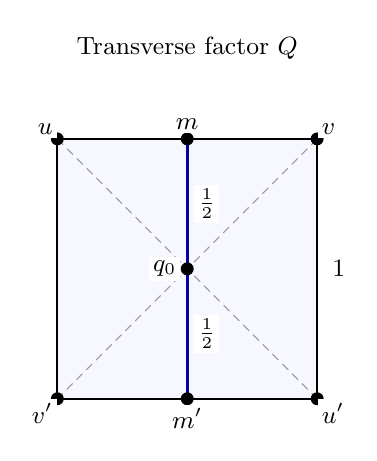
\begin{tikzpicture}[x=3.3cm,y=3.3cm,
  square vertex/.style={circle,fill=black,inner sep=1.65pt},
  square label/.style={font=\small,fill=white,inner sep=1.5pt}]
  \coordinate (u) at (-.5,.5);
  \coordinate (v) at (.5,.5);
  \coordinate (up) at (.5,-.5);
  \coordinate (vp) at (-.5,-.5);
  \coordinate (m) at (0,.5);
  \coordinate (mp) at (0,-.5);
  \coordinate (q) at (0,0);
  \fill[blue!3] (u)--(v)--(up)--(vp)--cycle;
  \draw[draw=black!40,densely dashed] (u)--(up) (v)--(vp);
  \draw[line width=.85pt] (u)--(v)--(up)--(vp)--cycle;
  \draw[draw=blue!65!black,line width=1.2pt] (m)--(mp);
  \foreach \P in {u,v,up,vp,m,mp,q}
    \node[square vertex] at (\P) {};
  \node[square label,anchor=south east] at (u) {$u$};
  \node[square label,anchor=south west] at (v) {$v$};
  \node[square label,anchor=north west] at (up) {$u'$};
  \node[square label,anchor=north east] at (vp) {$v'$};
  \node[square label,anchor=south] at (0,.52) {$m$};
  \node[square label,anchor=north] at (0,-.52) {$m'$};
  \node[square label,anchor=east] at (-.025,0) {$q_0$};
  \node[square label,anchor=west] at (.025,.25) {$\frac12$};
  \node[square label,anchor=west] at (.025,-.25) {$\frac12$};
  \node[square label,anchor=west] at (.54,0) {$1$};
  \node[font=\small] at (0,.85) {Transverse factor $Q$};
\end{tikzpicture}
\end{minipage}\hfill
\begin{minipage}[c]{.53\textwidth}
\centering
\begin{tikzpicture}[x=2.05cm,y=1cm,
  axis label/.style={font=\small,fill=white,inner sep=1.5pt}]
  \draw[{Stealth[length=4pt]}-{Stealth[length=4pt]},line width=.7pt]
    (-1.22,0)--(1.22,0);
  \foreach \x in {-1,0,1}\fill (\x,0) circle[radius=1.65pt];
  \node[axis label,anchor=south] at (-1,.07) {$M_D$};
  \node[axis label,anchor=south] at (1,.07) {$M_C$};
  \node[axis label,anchor=north] at (0,-.07) {$0_T$};
  \node[font=\small] at (0,.9) {Axis $\ell=\mathbb R\times\{q_0\}$};
\end{tikzpicture}
\par\smallskip
$P(\ell)\cong\mathbb R\times Q$\par\medskip
$M_A=2(0,m),\qquad M_B=2(0,m')$
\end{minipage}
\caption{The final contradiction takes place in the transverse factor after
splitting off the $M_C,M_D$ axis.  The cyclically ordered points $u,v,u',v'$
form a flat unit square in $Q$, with common diagonal midpoint $q_0$.
The opposite-side midpoints $m,m'$ are distance $1/2$ from $q_0$ and distance
$1$ apart.  Dilation in the original tangent cone $T$ therefore makes
$M_A=2(0,m)$ and $M_B=2(0,m')$ antipodal unit vectors.  The panels display
the two distinct factors of the parallel set.}
\label{fig:transverse-square}
\end{figure}
